\documentclass[14pt]{beamer}
\usepackage[utf8]{inputenc}
\usepackage{graphicx}
\usepackage{tikz}
\usepackage{booktabs}
\usepackage{pgfgantt}
\usepackage{array}
\usepackage{xcolor}
\usetikzlibrary{shapes.geometric, arrows, positioning, calc}

% Theme settings
\usetheme{Madrid}
\usecolortheme{default}
\setbeamertemplate{navigation symbols}{}

% Custom colors
\definecolor{navyblue}{RGB}{0, 51, 102}
\definecolor{lightgray}{RGB}{245, 245, 245}
\setbeamercolor{title}{fg=white, bg=navyblue}
\setbeamercolor{frametitle}{fg=white, bg=navyblue}
\setbeamercolor{block title}{fg=white, bg=navyblue}
\setbeamercolor{structure}{fg=navyblue}

% Define colors
\definecolor{processblue}{RGB}{70, 130, 200}
\definecolor{decisionorange}{RGB}{255, 165, 0}
\definecolor{startgreen}{RGB}{50, 150, 50}
\definecolor{endred}{RGB}{200, 50, 50}
\definecolor{taskcolor}{RGB}{52, 152, 219}
\definecolor{completedcolor}{RGB}{46, 204, 113}
\definecolor{inprogresscolor}{RGB}{241, 196, 15}
\definecolor{milestonecolor}{RGB}{155, 89, 182}

\tikzstyle{startstop} = [rectangle, rounded corners, minimum width=3cm, minimum height=1cm, text centered, text width=3.5cm, draw=black, fill=startgreen!20, font=\small]
\tikzstyle{process} = [rectangle, minimum width=3cm, minimum height=1cm, text centered, text width=3.5cm, draw=black, fill=processblue!20, font=\small]
\tikzstyle{decision} = [diamond, minimum width=3cm, minimum height=1cm, text centered, text width=3cm, draw=black, fill=decisionorange!20, font=\small, aspect=2]
\tikzstyle{arrow} = [thick,->,>=stealth]
\tikzstyle{connector} = [thick,->,>=stealth, dashed]

% Title page
\title{AS-IS vs TO-BE Process Overview \\ \& Automation Roadmap}
\subtitle{Warehouse Management System}
\date{February 25, 2026}

\begin{document}

% Title frame
\begin{frame}
  \titlepage
\end{frame}

% Agenda
\begin{frame}{Agenda}
  \begin{itemize}
    \item AS-IS process overview
    \item Identified gaps
    \item Proposed TO-BE process \& automation scope
    \item Assumptions \& dependencies
    \item Next steps \& validation
  \end{itemize}
\end{frame}

% AS-IS Process Overview
\begin{frame}{AS-IS Process Overview}
  \begin{itemize}
    \item Predominantly manual or semi-manual operations
    \item Limited system-driven controls
    \item High dependency on user intervention
    \item Limited real-time visibility
  \end{itemize}
\end{frame}

% Process Flow Diagrams - Placeholder
\begin{frame}{FG Production Floor to Warehouse Operation Process Flow (AS-IS)}
  \begin{center}
    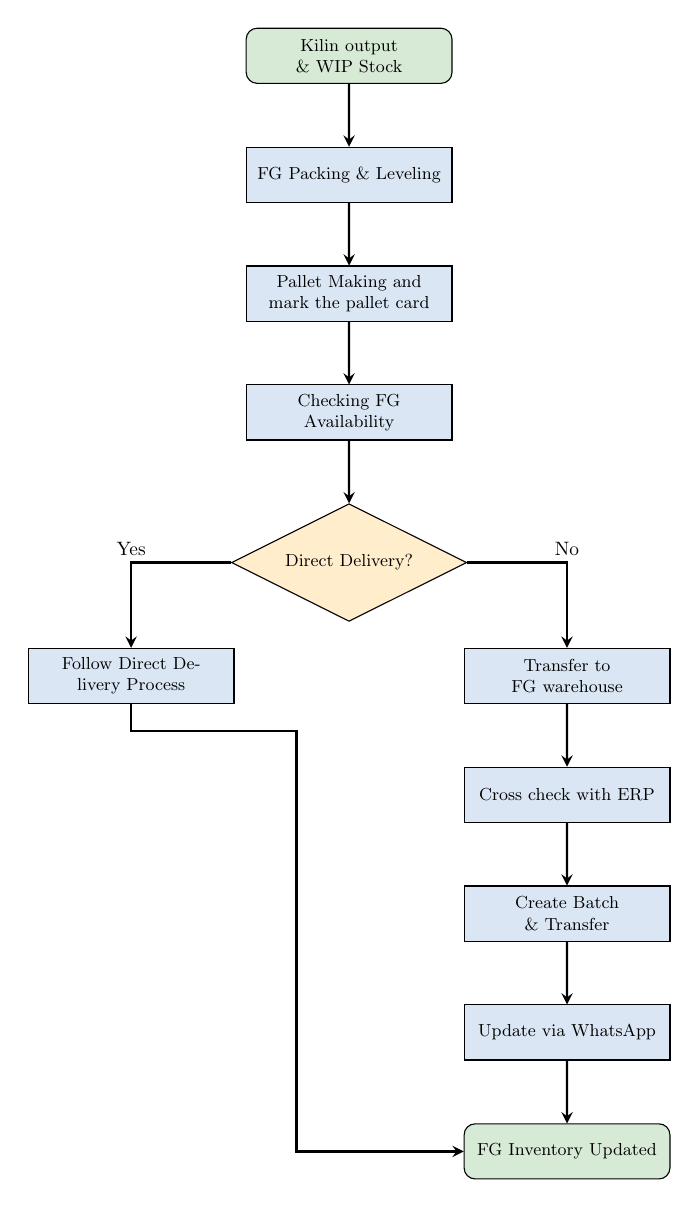
\begin{tikzpicture}[node distance=0.8cm, auto, scale=0.7, every node/.style={scale=0.7}]
      \node[startstop] (start) {Kilin output \& WIP Stock};
      \node[process, below=of start] (packing) {FG Packing \& Leveling};
      \node[process, below=of packing] (pallet) {Pallet Making and mark the pallet card};
      \node[process, below=of pallet] (checking) {Checking FG Availability};
      \node[decision, below=of checking] (decision) {Direct Delivery?};
      \node[process, below left=1cm of decision] (direct) {Follow Direct Delivery Process};
      \node[process, below right=1cm of decision] (transfer) {Transfer to FG warehouse};
      \node[process, below=of transfer] (crosscheck) {Cross check with ERP};
      \node[process, below=of crosscheck] (batch) {Create Batch \& Transfer};
      \node[process, below=of batch] (whatsapp) {Update via WhatsApp};
      \node[startstop, below=of whatsapp] (end) {FG Inventory Updated};

      \draw[arrow] (start) -- (packing);
      \draw[arrow] (packing) -- (pallet);
      \draw[arrow] (pallet) -- (checking);
      \draw[arrow] (checking) -- (decision);
      \draw[arrow] (decision) -| node[above] {Yes} (direct);
      \draw[arrow] (decision) -| node[above] {No} (transfer);
      \draw[arrow] (direct) |- ++(3cm,-1cm) |- (end);
      \draw[arrow] (transfer) -- (crosscheck);
      \draw[arrow] (crosscheck) -- (batch);
      \draw[arrow] (batch) -- (whatsapp);
      \draw[arrow] (whatsapp) -- (end);
    \end{tikzpicture}
  \end{center}
\end{frame}

\begin{frame}{FG Sales Order to Delivery Process Flow (AS-IS)}
  \begin{center}
    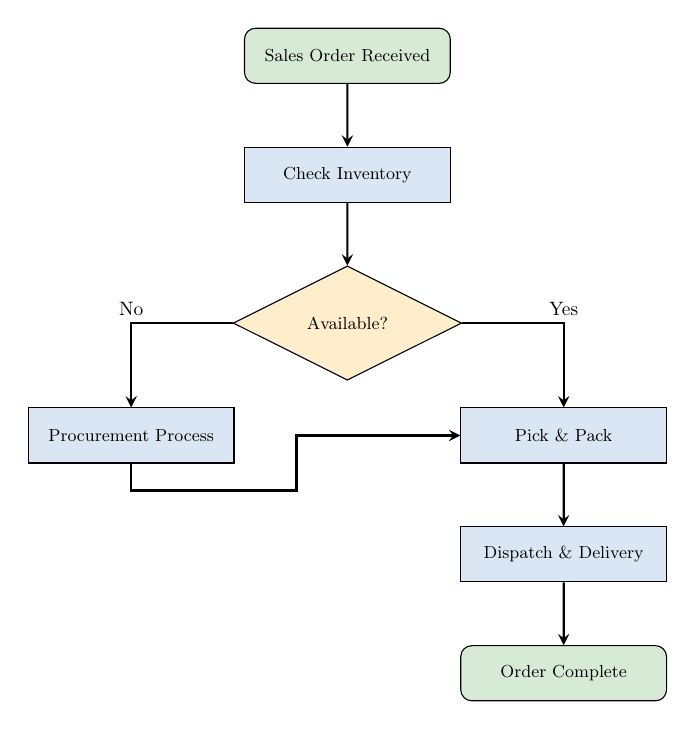
\begin{tikzpicture}[node distance=0.8cm, auto, scale=0.7, every node/.style={scale=0.7}]
      \node[startstop] (start) {Sales Order Received};
      \node[process, below=of start] (check) {Check Inventory};
      \node[decision, below=of check] (avail) {Available?};
      \node[process, below left=1cm of avail] (procure) {Procurement Process};
      \node[process, below right=1cm of avail] (pick) {Pick \& Pack};
      \node[process, below=of pick] (dispatch) {Dispatch \& Delivery};
      \node[startstop, below=of dispatch] (end) {Order Complete};

      \draw[arrow] (start) -- (check);
      \draw[arrow] (check) -- (avail);
      \draw[arrow] (avail) -| node[above] {No} (procure);
      \draw[arrow] (avail) -| node[above] {Yes} (pick);
      \draw[arrow] (procure) |- ++(3cm,-1cm) |- (pick);
      \draw[arrow] (pick) -- (dispatch);
      \draw[arrow] (dispatch) -- (end);
    \end{tikzpicture}
  \end{center}
\end{frame}

% AS-IS Pain Points
\begin{frame}{AS-IS Pain Points}
  \begin{block}{Operational Issues}
    \begin{itemize}
      \item Manual data entry and errors
      \item Delayed inventory updates
    \end{itemize}
  \end{block}
  \begin{block}{System Issues}
    \begin{itemize}
      \item Inefficient warehouse movement
      \item Limited traceability
    \end{itemize}
  \end{block}
\end{frame}

% Identified Gaps
\begin{frame}{Identified Gaps}
  \begin{alertblock}{Critical Findings}
    \begin{itemize}
      \item No system-enforced process control
      \item Limited real-time inventory accuracy
      \item Operator-dependent productivity
      \item Not scalable for future growth
    \end{itemize}
  \end{alertblock}
\end{frame}

% TO-BE Vision
\begin{frame}{TO-BE Vision}
  \begin{block}{Future State Objectives}
    \begin{itemize}
      \item \textbf{System-driven} standardized processes
      \item \textbf{Automation-enabled} operations
      \item \textbf{Real-time} inventory visibility
      \item \textbf{Scalable} and \textbf{audit-ready} design
    \end{itemize}
  \end{block}
\end{frame}

% Proposed TO-BE Process
\begin{frame}{Proposed TO-BE Process}
  \begin{itemize}
    \item Digitally enabled inbound to dispatch
    \item Barcode / QR-based tracking
  \end{itemize}
  \begin{itemize}
    \item Rule-based inventory movement
    \item Integrated dashboards and reports
  \end{itemize}
\end{frame}

% TO-BE Process Flow
\begin{frame}{TO-BE Process Flow Diagram}

\end{frame}

% Automation Scope
\begin{frame}{Automation \& System Enablement Scope}
  \begin{block}{Technical Implementation}
    \begin{itemize}
      \item WMS configuration
      \item Barcode / QR / RFID integration
      \item Mobile / RF operations
      \item Validation and exception handling
    \end{itemize}
  \end{block}
\end{frame}

% Business Benefits
\begin{frame}{Business Benefits}
  \begin{itemize}
    \item Improved accuracy and control
    \item Reduced operational cycle time
    \item Better space utilization
    \item Enhanced decision making
  \end{itemize}
\end{frame}

% Key Assumptions
\begin{frame}{Key Assumptions}
  \begin{exampleblock}{Prerequisites}
    \begin{itemize}
      \item Clean and defined master data
      \item Warehouse Layout designed properly for WMS
      \item Hardware and network availability
      \item Business user availability
      \item SOP alignment
    \end{itemize}
  \end{exampleblock}
\end{frame}

% Dependencies
\begin{frame}{Dependencies \& Considerations}
  \begin{alertblock}{Critical Dependencies}
    \begin{itemize}
      \item ERP/WMS readiness
      \item Infrastructure stability
      \item Change management and training
    \end{itemize}
  \end{alertblock}
\end{frame}

% Project Plan Table
\begin{frame}{Project Plan}
  \tiny
  \begin{tabular}{|p{1.8cm}|p{1.2cm}|p{1.2cm}|p{0.8cm}|p{1.5cm}|p{1.2cm}|}
    \hline
    \textbf{Task} & \textbf{Start} & \textbf{End} & \textbf{Dur} & \textbf{Dependency} & \textbf{Status} \\
    \hline
    Project Kickoff & 01-Feb & 05-Feb & 4 & - & Completed \\
    \hline
    AS-IS Process Study & 01-Feb & 22-Feb & 21 & Kickoff & In-Progress \\
    \hline
    Infrastructure & 03-Feb & 15-Feb & 12 & - & Completed \\
    \hline
    TO-BE Blueprint & 15-Feb & 10-Mar & 23 & AS-IS & Planned \\
    \hline
    Inbound Setup & 06-Mar & 20-Mar & 15 & Blueprint & Planned \\
    \hline
    Put-away Rules & 10-Mar & 25-Mar & 16 & Inbound & Planned \\
    \hline
    Picking \& Wave & 15-Mar & 30-Mar & 16 & Put-away & Planned \\
    \hline
    Shipping & 12-Mar & 25-Mar & 14 & Picking & Planned \\
    \hline
    RF \& Barcode & 10-Mar & 30-Mar & 21 & Setup & Planned \\
    \hline
    Data Cleansing & 01-Mar & 30-Mar & 30 & - & Planned \\
    \hline
    Unit Testing & 10-Mar & 25-Mar & 16 & Config & Planned \\
    \hline
    UAT \& Training & 10-Apr & 20-Apr & 11 & Testing & Planned \\
    \hline
    Cutover Prep & 20-Apr & 30-Apr & 11 & UAT & Planned \\
    \hline
    Hypercare & 25-Apr & 30-Apr & 6 & Cutover & Planned \\
    \hline
    Go-Live & 02-May & 02-May & 0 & Cutover & Milestone \\
    \hline
  \end{tabular}

  \vspace{0.3cm}
  \begin{center}
    \tiny
    \colorbox{completedcolor}{\hspace{0.2cm}} Completed \hspace{0.2cm}
    \colorbox{inprogresscolor}{\hspace{0.2cm}} In Progress \hspace{0.2cm}
    \colorbox{taskcolor}{\hspace{0.2cm}} Planned \hspace{0.2cm}
    \colorbox{milestonecolor}{\hspace{0.2cm}} Milestone
  \end{center}
\end{frame}

% Simplified Gantt Chart using TikZ (FIXED - No pgfgantt)
\begin{frame}{Project Timeline - Gantt Chart}
  \begin{center}
    \resizebox{0.9\textwidth}{!}{%
      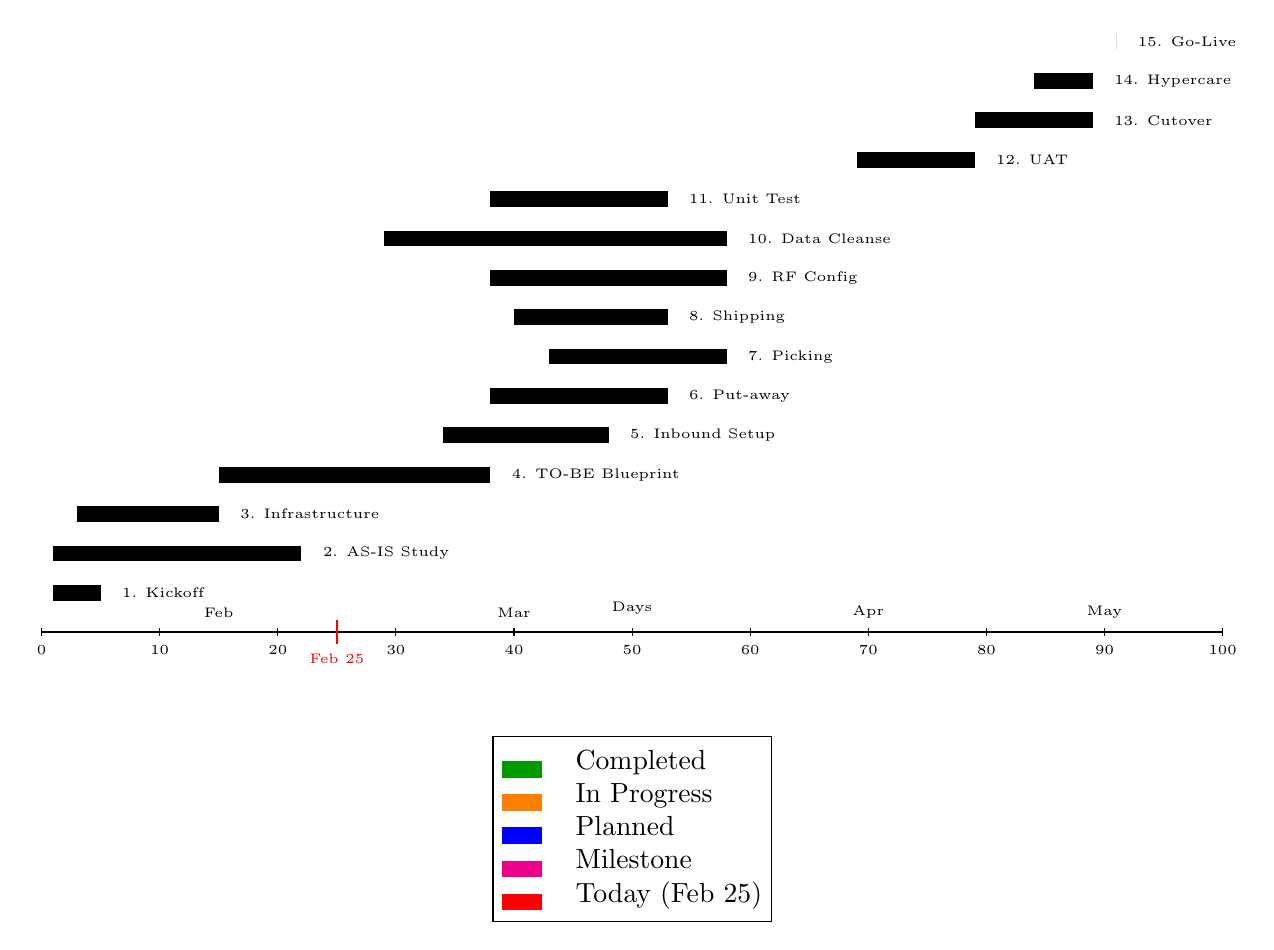
\begin{tikzpicture}[x=0.15cm, y=0.5cm]
        % Timeline
        \draw[thick] (0,0) -- (100,0);
        \foreach \x in {0,10,20,30,40,50,60,70,80,90,100}
        \draw (\x,0.1) -- (\x,-0.1) node[below] {\tiny \x};
        \node[above] at (50,0.2) {\tiny Days};

        % Month markers
        \draw[red, thick] (25,0.3) -- (25,-0.3) node[below] {\tiny Feb 25};
        \node at (15,0.5) {\tiny Feb};
        \node at (40,0.5) {\tiny Mar};
        \node at (70,0.5) {\tiny Apr};
        \node at (90,0.5) {\tiny May};

        % Tasks (y positions)
        \foreach \y/\task/\start/\end/\color in {
          1/1. Kickoff/1/5/completed,
          2/2. AS-IS Study/1/22/inprogress,
          3/3. Infrastructure/3/15/completed,
          4/4. TO-BE Blueprint/15/38/planned,
          5/5. Inbound Setup/34/48/planned,
          6/6. Put-away/38/53/planned,
          7/7. Picking/43/58/planned,
          8/8. Shipping/40/53/planned,
          9/9. RF Config/38/58/planned,
          10/10. Data Cleanse/29/58/planned,
          11/11. Unit Test/38/53/planned,
          12/12. UAT/69/79/planned,
          13/13. Cutover/79/89/planned,
          14/14. Hypercare/84/89/planned,
          15/15. Go-Live/91/91/milestone
        }{
          \ifx\color\color
            \ifx\color\milestone
              \fill[magenta] (\start,\y) circle (2pt);
              \node[right] at (\start+1,\y) {\tiny \task};
            \else
              \ifx\color\completed
                \fill[green!60!black] (\start,\y-0.2) rectangle (\end,\y+0.2);
              \else
                \ifx\color\inprogress
                  \fill[orange] (\start,\y-0.2) rectangle (\end,\y+0.2);
                \else
                  \fill[blue] (\start,\y-0.2) rectangle (\end,\y+0.2);
                \fi
              \fi
              \node[right] at (\end+1,\y) {\tiny \task};
            \fi
          \fi
        }

        % Legend
        \node[draw, fill=white] at (50,-5) {
            \begin{tabular}{@{}ll@{}}
              \colorbox{green!60!black}{\hspace{0.3cm}} & Completed \\
              \colorbox{orange}{\hspace{0.3cm}} & In Progress \\
              \colorbox{blue}{\hspace{0.3cm}} & Planned \\
              \colorbox{magenta}{\hspace{0.3cm}} & Milestone \\
              \colorbox{red}{\hspace{0.3cm}} & Today (Feb 25)
            \end{tabular}
          };
      \end{tikzpicture}
    }
  \end{center}
\end{frame}

% Next Steps
\begin{frame}{Next Steps}
  \begin{enumerate}
    \item Validate TO-BE scope
    \item Confirm automation priorities
    \item Finalize implementation roadmap
    \item Client sign-off
  \end{enumerate}
\end{frame}

% Validation Required
\begin{frame}{Validation Required}
  \begin{itemize}
    \item Process alignment confirmation
    \item Automation scope approval
    \item Assumptions acceptance
    \item Go-ahead for next phase
  \end{itemize}
\end{frame}

% Thank You
\begin{frame}{Thank You}
  \begin{center}
    \vspace{1cm}
    {\Huge \textcolor{navyblue}{Thank You}}

    \vspace{1cm}
    \textcolor{navyblue}{Questions?}
  \end{center}
\end{frame}

\end{document}
